\documentclass[french]{article}

\usepackage{MyPack2}
\geometry{top=2cm, bottom=2cm, left=3cm, right=3cm}
\title{TL d'ELAN\\Conception d'un AO}
\author{Binôme A11 \\ \bsc{Simon} Léo, \bsc{Levy--Falk} Hugo}
\date{\today}

\begin{document}
	\maketitle
	
	\tableofcontents
	\listoffigures
	\newpage
	
	\initPage{TL - SIG1}{\today}{\bsc{Simon}, \bsc{Levy--Falk}}

\part*{ Introduction}

Le but de ce TL est de concevoir un amplificateur opérationnel possédant les spécifications suivantes :

\begin{itemize}
	\item Décalage statique de courant nul;
	\item Transconductance minimale de 10mS;
	\item Excursion de sortie sur + ou - 1V sur une résistance de charge de $10k\Omega$;
	\item Tensions d'alimentation $V_{DD}=2.5V$ et $V_{SS}=-2.5V$.
\end{itemize}

Avec :

\begin{itemize}
	\item Pour les NMOS : $V_{TN}=0.74V$ et $\mu_N C_{oxN} = 75 \mu A/V²$;
	\item Pour les PMOS : $V_{TN}=-0.75V$ et $\mu_N C_{oxN} = 25 \mu A/V²$.
\end{itemize}

On étudie en premier lieu le modèle du NMOS en vérifiant que faire varier le potentiel du substrat revient à faire varier le $V_T$ du transistor, comme le montre la figure \ref{caracMOS}.

\begin{figure}[h!]
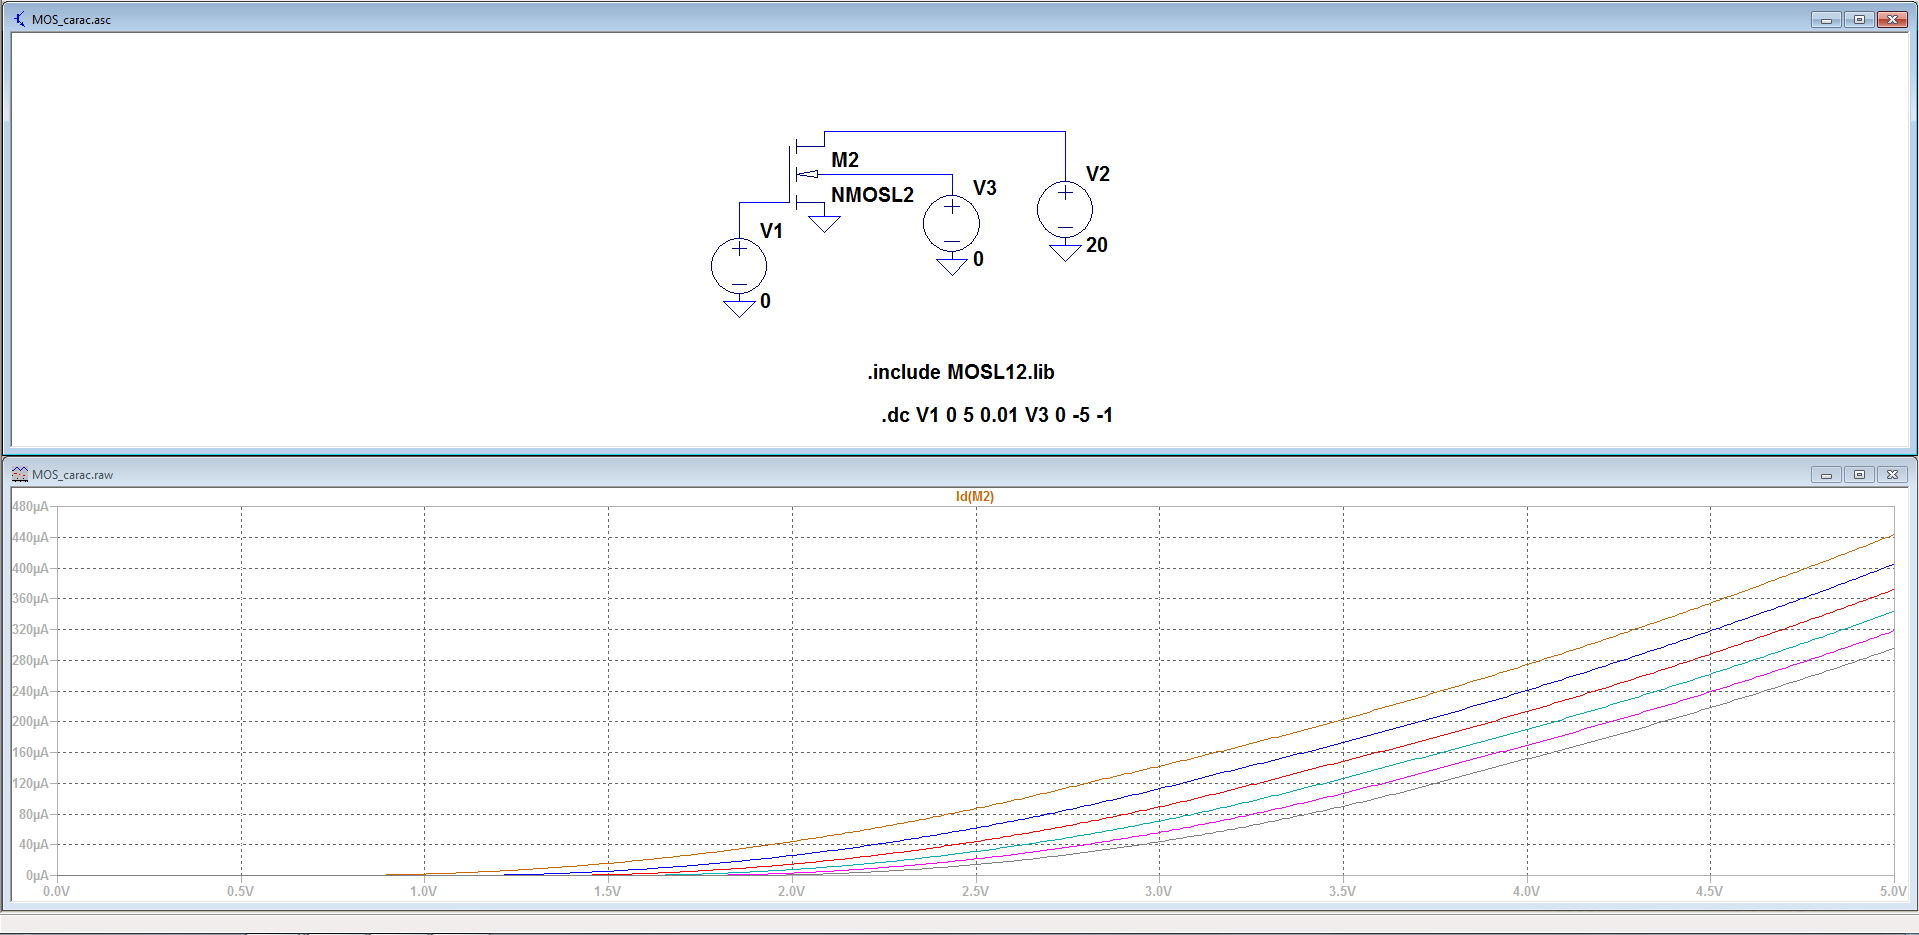
\includegraphics[width=\textwidth]{images/MOSCarac.PNG}
\caption{La variation de $V_3$ décale la courbe.}
\label{caracMOS}
\end{figure}

\newpage
\part{ Étage 1}
\label{part:etage1}
Le premier étage constitue un amplificateur SCV $\rightarrow$ I dont on trouvera le schéma sur la figure \ref{circuit}. Il est constitué d'un montage différentiel, d'un miroir de courant et d'une source de courant. Il faut dimensionner les transistors qui composent l'amplificateur.

\begin{figure}[h!]
	\centering
	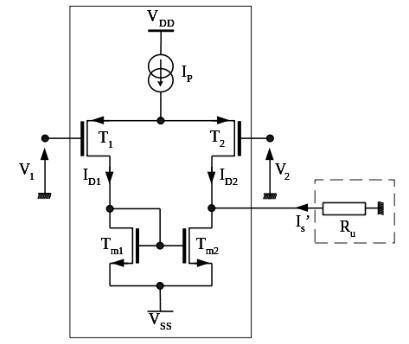
\includegraphics[height=0.25\textheight]{images/circuit.png}
	\caption{Schéma de l'amplificateur SCV $\rightarrow$ I}
	\label{circuit}
\end{figure}

\section{ Amplificateur différentiel et miroir de courant}

\subsection{ Prédéterminations}

\subsubsection{ Montage différentiel}

On a un montage différentiel avec miroir de courant. Le gain $G$ d'un tel montage vérifie $G=-g_m$. En développant autour du point de fonctionnement $V_{10} = V_{20} = 0V$ avec $I_p = 20 \mu A$, on a alors :
\begin{equation}
-G = g_m = k' \frac{W}{L} (V_{GS} - V_T) = \sqrt{I_p k' \frac{W}{P}} \label{eq:GainT}
\end{equation}

Or on souhaite :
\begin{itemize}
	\item $g_m = 140 \mu S$;
	\item $I_p = 20 \mu A$;
	\item $L = 20 \mu A$;
	\item $k' = 25 \mu A . V^{-2}$.
\end{itemize}

On peut alors déterminer la largeur des MOS en résolvant l'équation \ref{eq:GainT} :
\[
\boxed{W_{T1} = W_{T2} = 7.84 \times 10^{-5} m}
\]

\subsubsection{ Miroir de courant}

Il y a un miroir de courant couplé avec le montage différentiel. Pour dimensionner les transistors $T_{m1}$ et $T_{m2}$, on les polarise autour de $V_{GS0}=1.2V$. On a alors :
\begin{equation}
  \frac{I_p}{2} = I_D = \frac{1}{2} k' \frac{W}{L} (V_{GS} - V_T)^2 \label{eq:PolariseW}
\end{equation}

En résolvant l'équation \ref{eq:PolariseW}, on a alors :
\[
\boxed{W_{T_{m1}} = W_{T_{m1}} =  2.52 \times 10^{-6} m}
\]

\subsubsection{ Carte des potentiels}

On souhaite déterminer le potentiel des points non connus. On a facilement le potentiel des grilles des $T_{mi}$ :
\[
V_{G_{T_m}} = V_{SS} + 1.2V = -1.3V
\]

Sur le transistor $T_1$, on a $V_{GS} = V_T + \sqrt{\frac{I_P \times L}{k' \times W}} = 8.93 \times 10 ^ {-1} V$. Il s'agit là du potentiel de la source des transistors $T_1$ et $T_2$.

\subsection{ Validation par simulation}

On souhaite maintenant valider les calculs avec une simulation. La figure \ref{level1} montre la simulation du montage en utilisant le level 1. On retrouve bien les valeurs de la prédétermination.

\begin{figure}[h!]
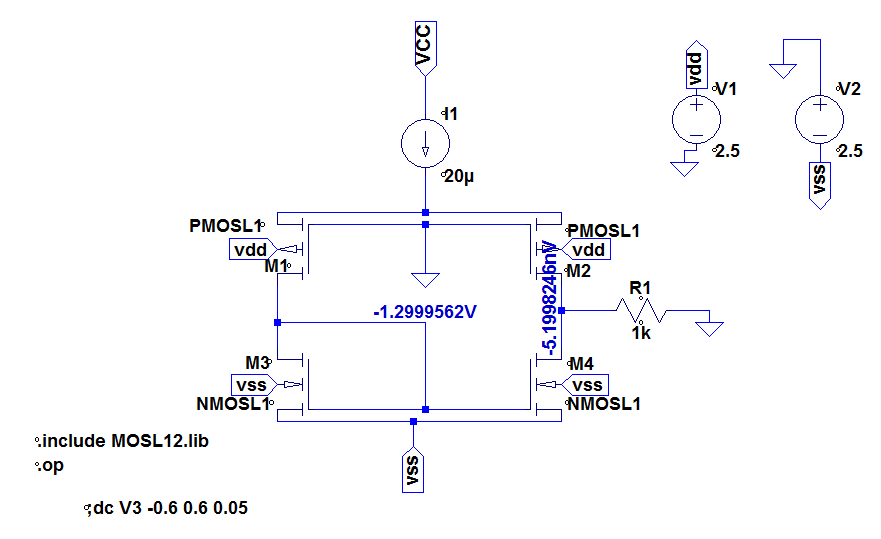
\includegraphics[width=\textwidth]{images/21Level1.PNG}
\caption{Montage avec le level 1}
\label{level1}
\end{figure}

On réalise ensuite la simulation avec le level 2. La figure \ref{level2} montre que ce modèle diffère des résultats de la prédétermination. On a notamment un offset en sortie.
\begin{figure}[h!]
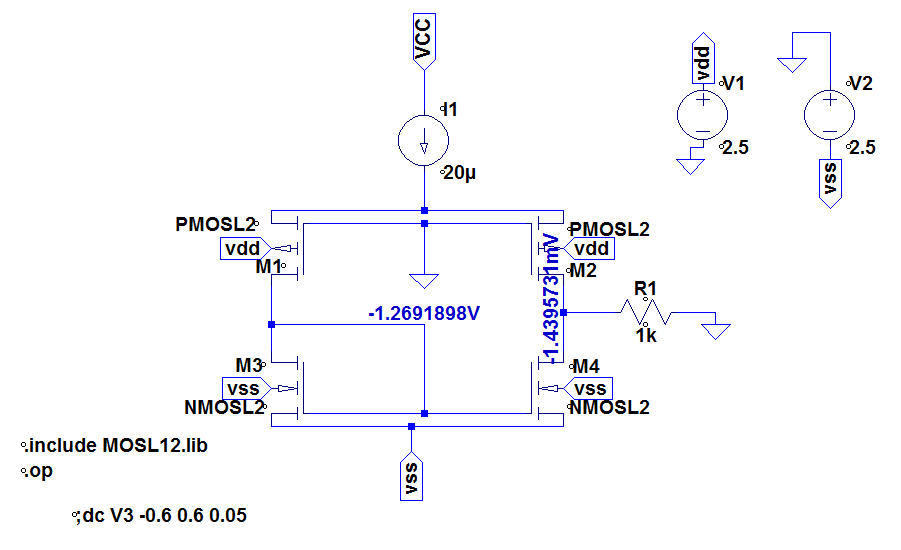
\includegraphics[width=\textwidth]{images/21Level2.PNG}
\caption{Montage avec le level 2}
\label{level2}
\end{figure}

On fait ensuite varier la différence de tension en entrée pour mesurer la transconductance de l'étage 1. La figure \ref{transcond} donne les résultats obtenus. On mesure la pente de la tangente en 0 de $I_D$ pour avoir la transconductance. On obtient avec le level 1 $140 \mu S$ et pour le level 2 $125 \mu S$. Ceci est encore dû au fait que le level 2 prend en compte plus de paramètres que le level 1. On voit aussi que la plage de fonctionnement linéaire est comprise entre $0.1V$ et $-0.1V$.

\begin{figure}[h!]
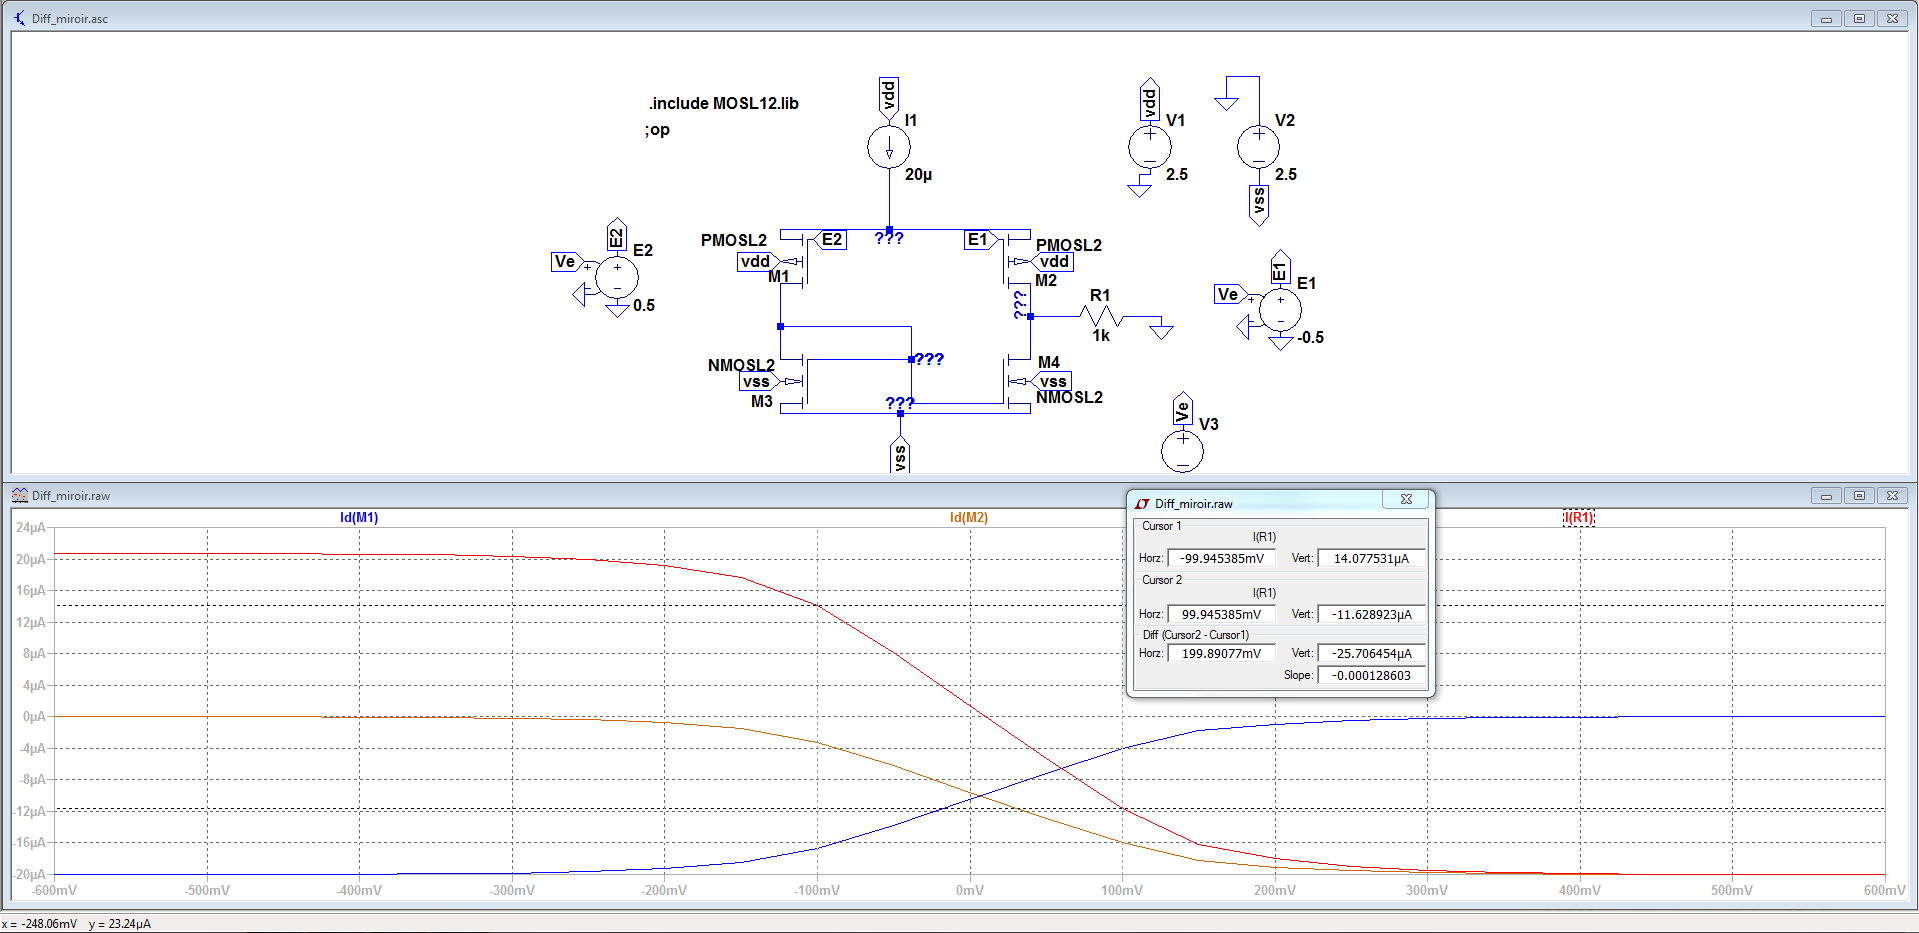
\includegraphics[width=\textwidth]{images/gmPincementLevel2.PNG}
\caption{Variations de $I_d1$ $I_d2$ et $I_R$ en fonction de $V_d$}
\label{transcond}
\end{figure}

\section{ Source de courant de polarisation}

Le schéma de l'étage 1 (représenté par la figure \ref{circuit}) fait appel à une source de courant. On se propose de la réaliser en suivant le modèle de la figure \ref{fig:sourceCourant}.

\begin{figure}[h!]
	\centering
	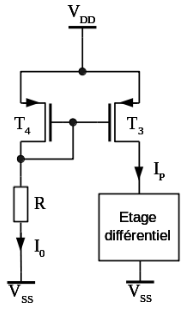
\includegraphics[height=0.25\textheight]{images/sourceCourant.png}
	\caption{Source de courant}
	\label{fig:sourceCourant}
\end{figure}


\subsection{ Prédéterminations}
On souhaite déterminer les valeurs associées aux composants de la source de courant. On sait que la résistance $R$ est traversée par un courant de $10 \mu A$. D'autre part puisque pour $T_4$ on a $V_{GS} = 1.25 V$, la tension aux bornes de la résistance vaut $3.75 V$. Ainsi
\[
\boxed{R = 3.75 \times 10 ^ {5} \Omega}
\]

Pour $T_4$ on a $I_D = 10 \mu A = \frac{1}{2} k' \frac{W}{L} (V_{GS} - V_T)^2$. On a donc, puisque le sujet fixe $L=5 \mu m$ :
\[
\boxed{W_{T_4} = 1.6 \times 10^{-5} m}
\]

De même:
\[
\boxed{W_{T_3} = 3.2 \times 10^{-5} m}
\]

On peut remplacer la résistance R par un PMOS dont la grille et le drain sont connectés. Avec la formule de la diode quadratique ($I_D = \frac{1}{2} k' \frac{W}{L} (V_{GS} - V_T)^2$), on a $W = 0.44 \mu A$. Le montage obtenu peut être retrouvé dans la figure \ref{sourceP}.

\subsection{ Validation par simulation}

On simule dans un premier temps le montage avec une résistance, comme montré dans la figure \ref{sourceRes}.

\begin{figure}[h!]
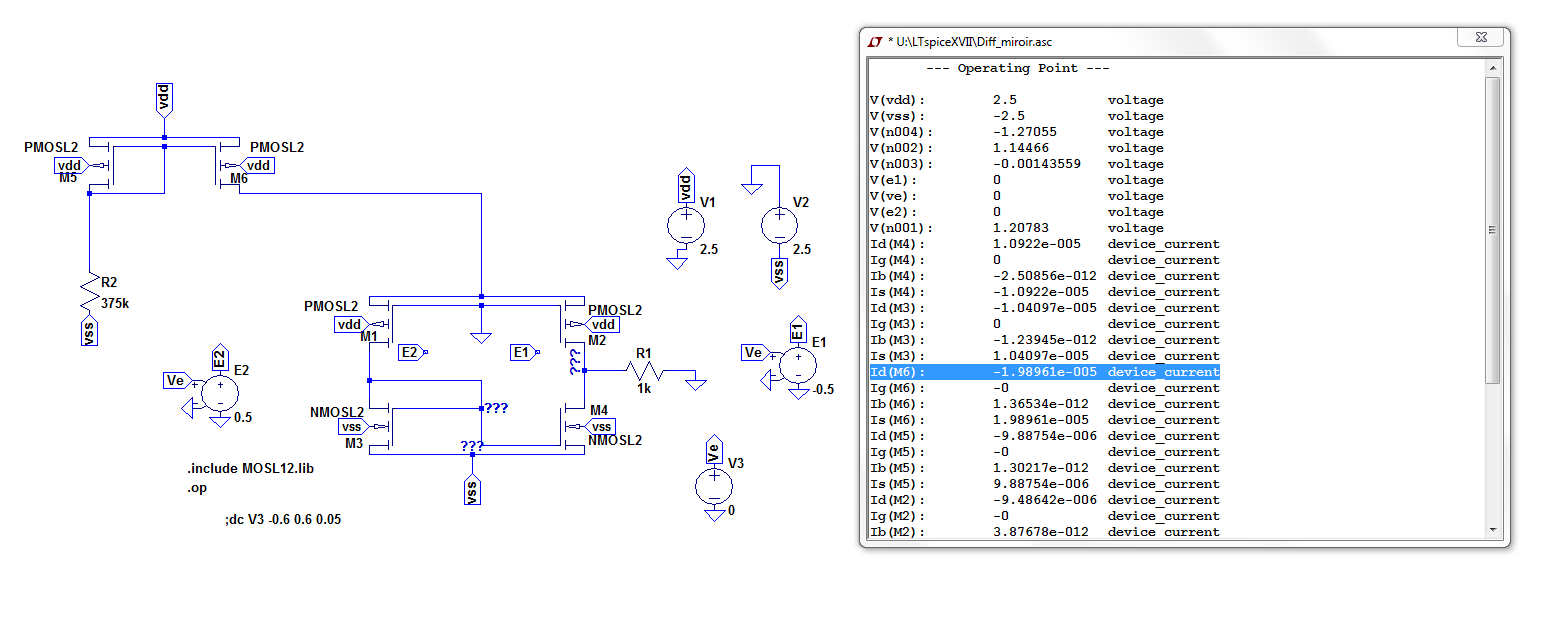
\includegraphics[width=\textwidth]{images/SourceCourrant.PNG}
\caption{Source de courant avec une résistance}
\label{sourceRes}
\end{figure}

On pourrait augmenter le W pour avoir pile $20 \mu A$ en sortie.

On simule ensuite avec notre solution constitué d'un PMOS (branché de manière à former une diode quadratique), comme montré dans la figure \ref{sourceP}. On ajustera la valeur du W afin d'avoir $20 \mu A$. On obtient alors :

\[
\boxed{W = 0.8 \mu m}
\]

\begin{figure}[h!]
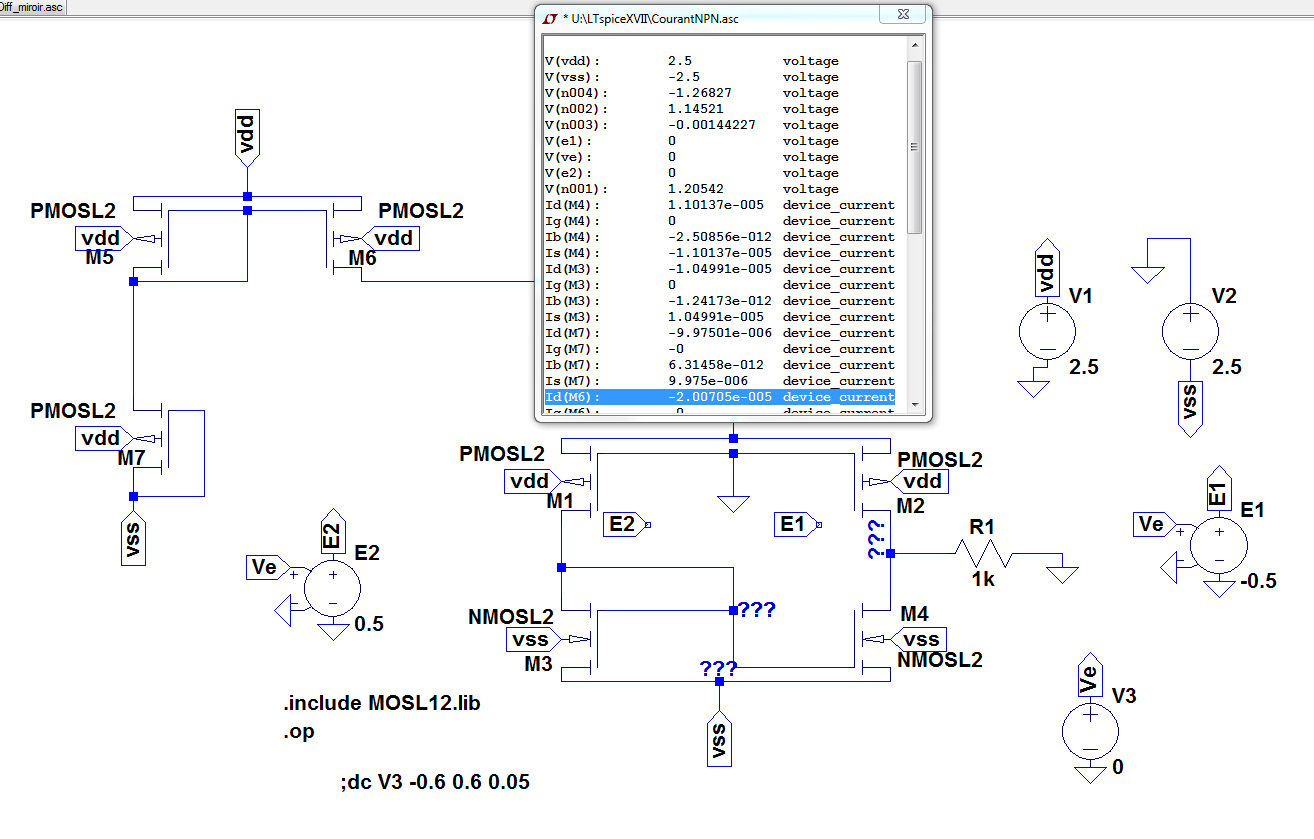
\includegraphics[width=\textwidth]{images/SourceNPN.PNG}
\caption{Source de courant avec un PMOS}
\label{sourceP}
\end{figure}

\FloatBarrier

 Dans la figure \ref{transcond2}, on réalise comme précédemment un tracé en faisant varier la différence de tension en entrée entre $-0.3 V$ et $0.3 V$. On calcule la transconductance de l'étage avec la pente de la tangente en 0. On trouve une transconductance d'environ $128 \mu S$, ce qui constitue une variation faible par rapport à ce que la source de courant parfaite offrait.

\begin{figure}[h!]
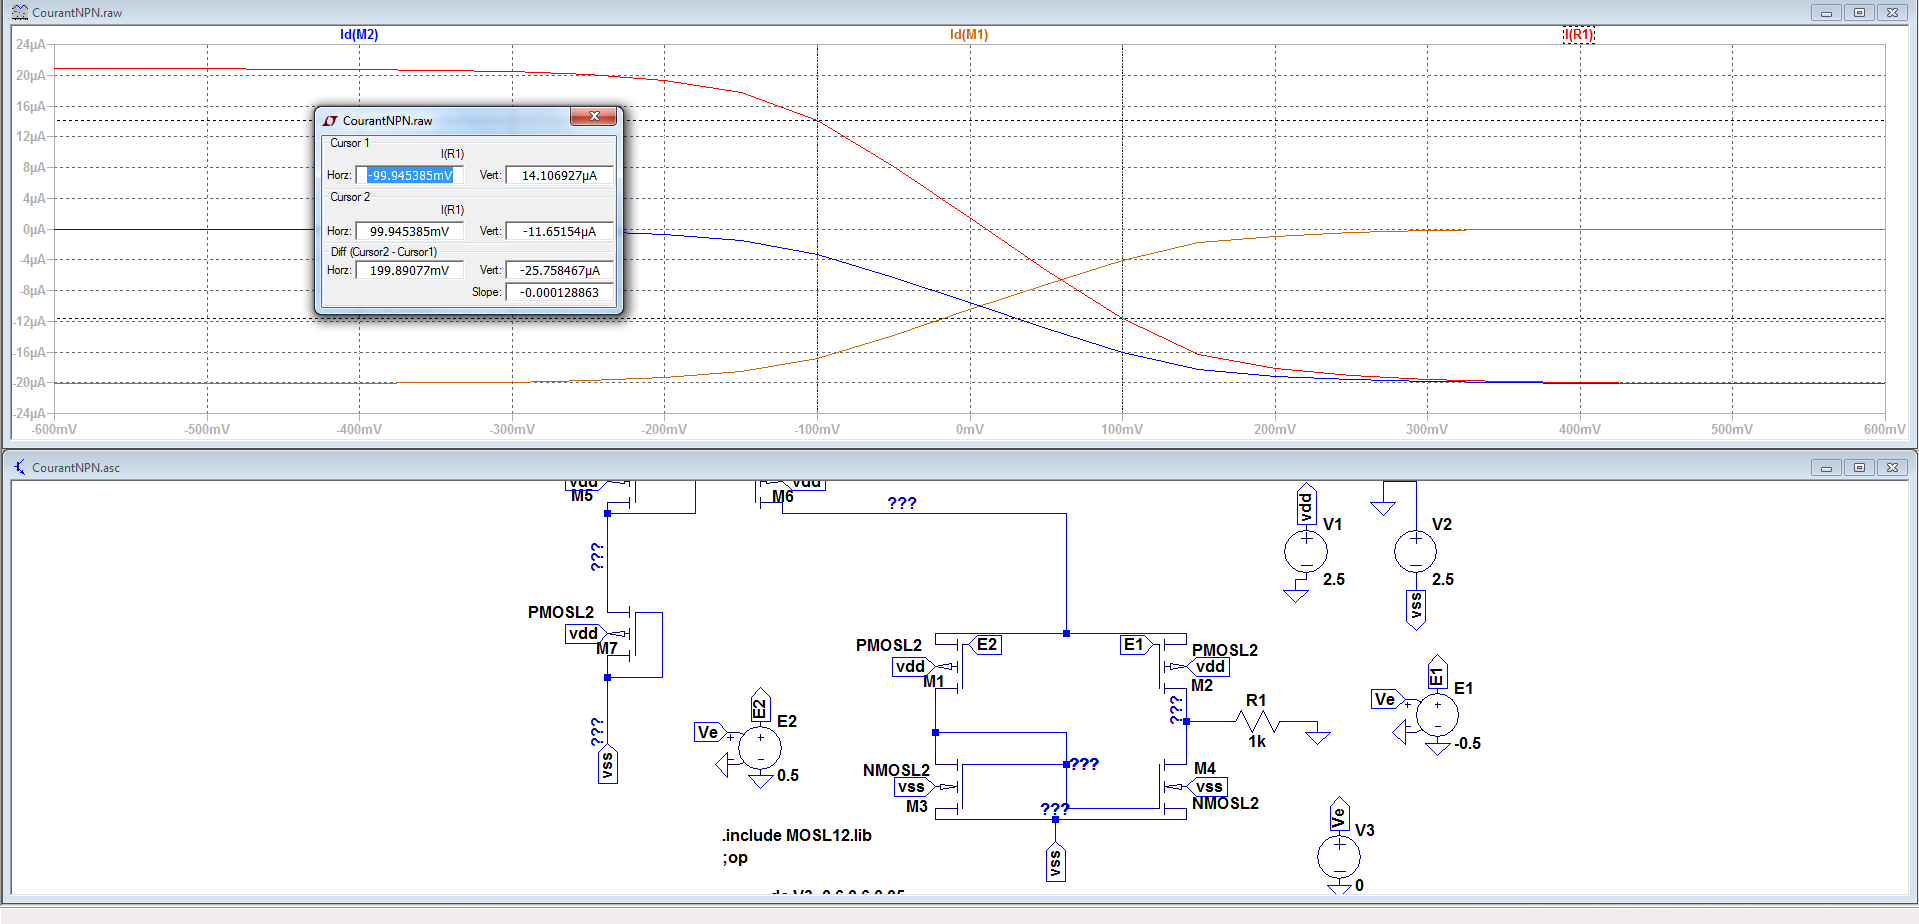
\includegraphics[width=\textwidth]{images/gmPincement222.PNG}
\caption{$I_{D1}$, $I_{D2}$ et $I_S$ en fonction de $V_e$}
\label{transcond2}
\end{figure}

\section{ Comportement en régime transitoire}
On veut étudier le comportement du montage en régime transitoire.
Pour cela, on impose $V_1=0$ et on prends un signal sinusoïdal de fréquence $10 kHz$. La figure \ref{transcond2} montre que la plage de fonctionnement linéaire se trouve entre $-0.1V$ et $0.1V$. Le résultat obtenu par simulation est donné par la figure \ref{transitoire}. On obtient alors une transconductance de $140 \; \mu S$

\begin{figure}[h!]
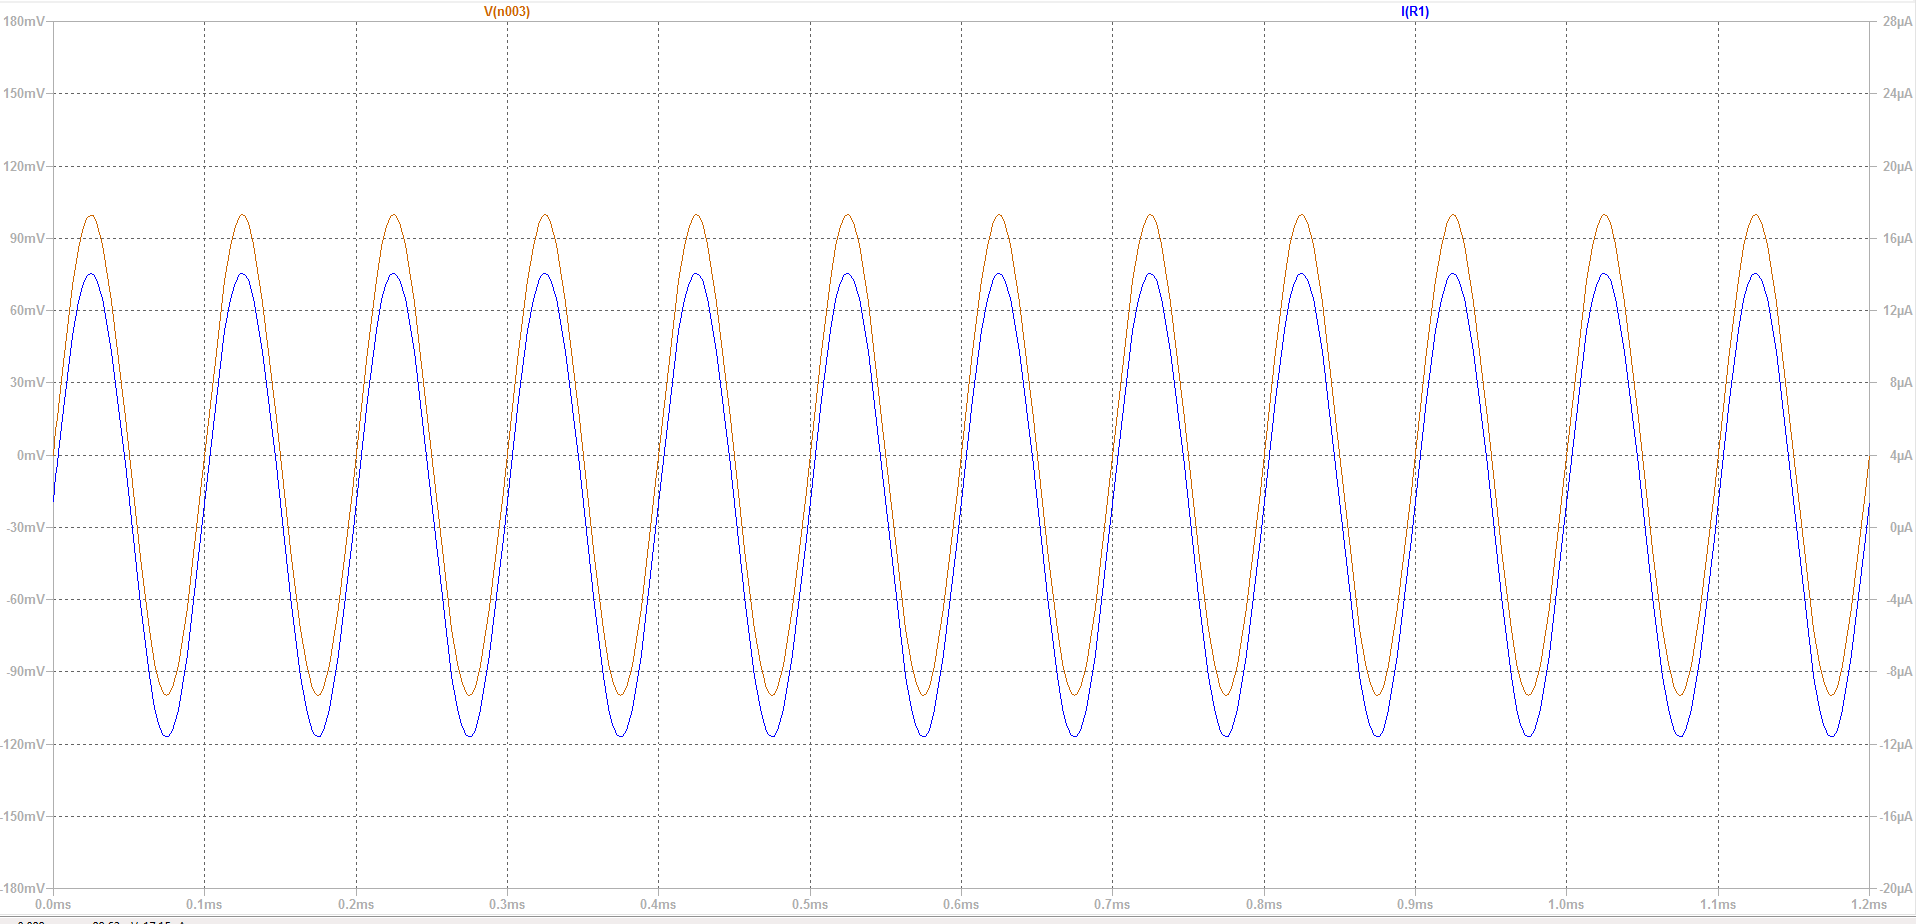
\includegraphics[width=\textwidth]{images/TransitoireLineaire.PNG}
\caption{Régime transitoire}
\label{transitoire}
\end{figure}

En multipliant $R_u$ par 1000, on obtient le chronogramme de la figure \ref{transitoire2}. On observe qu'on sort de la zone linéaire, on sature.

\begin{figure}[h!]
	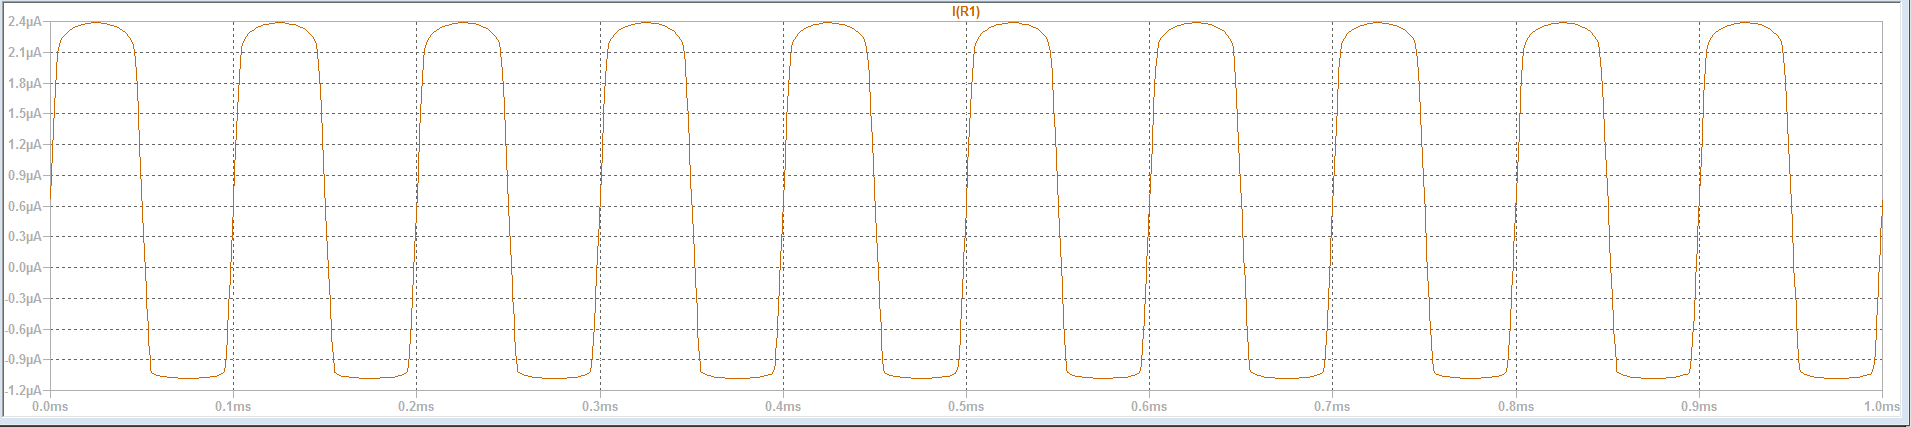
\includegraphics[width=\textwidth]{images/MulRuPar1000.PNG}
	\caption{Régime transitoire en multipliant $R_u$ par 1000}
	\label{transitoire2}
\end{figure}

Enfin avec $R_u = 1 \; k \Omega$ et en augmentant l'amplitude du signal d'entrée, on obtient le chronogramme de la figure \ref{transitoire3}. Là encore on sature.

\begin{figure}[h!]
	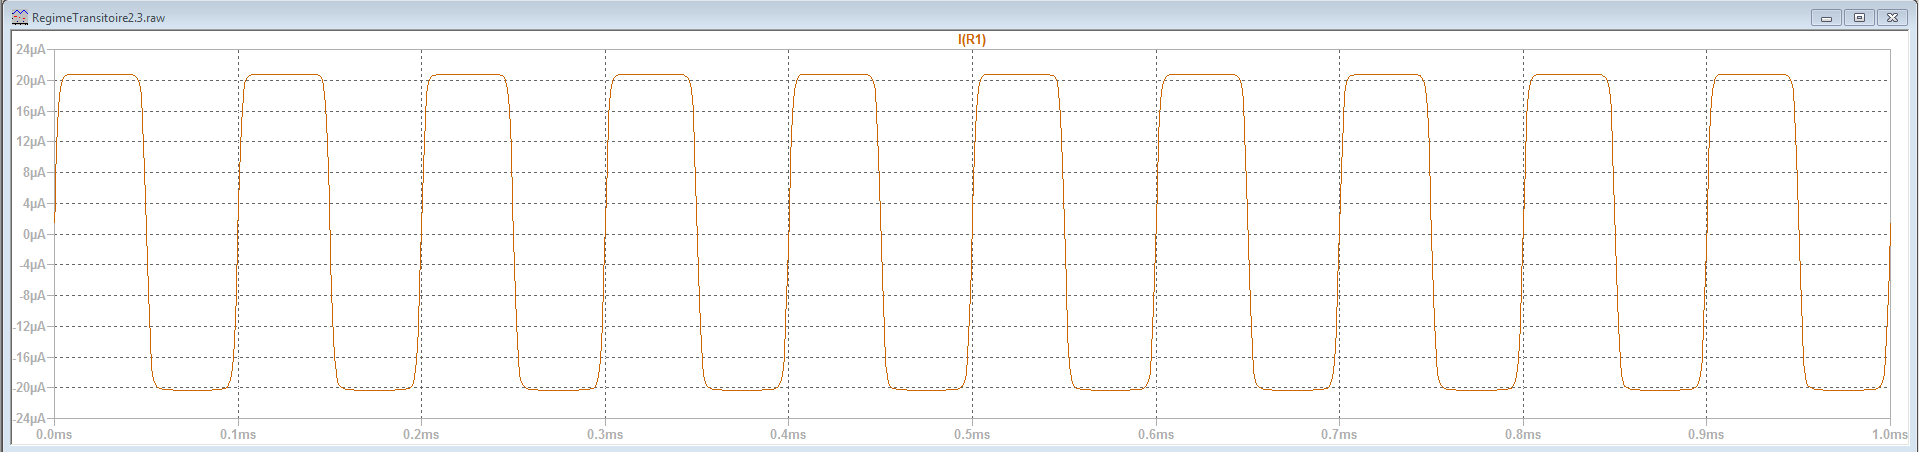
\includegraphics[width=\textwidth]{images/AugmentationSignalPar10.PNG}
	\caption{Régime transitoire en multipliant $R_u$ par 1000}
	\label{transitoire3}
\end{figure}

En conclusion pour rester dans la zone linéaire du montage, il faut une résistance de sortie peu élevée et une tension d'entrée qui permette de garder les MOS en régime de pincement.

\newpage
\part{Amplificateur opérationnel}

\section{Construction du schéma}

On complète le montage différentiel de la partie \ref{part:etage1} avec une SCV $\rightarrow$ I afin d'obtenir un gain important. Le schéma obtenu est donné à la figure \ref{fig:ampli}.


\begin{figure}[h!]
	\centering
	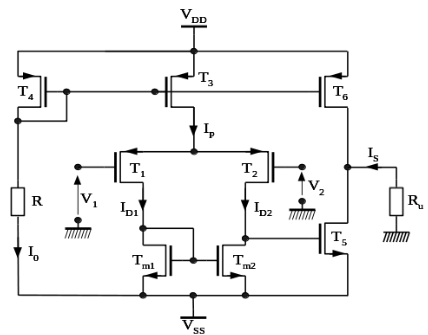
\includegraphics[height=0.25\textheight]{images/ampli.png}
	\caption{Schéma de l'amplificateur}
	\label{fig:ampli}
\end{figure}

\section{Prédéterminations}

On souhaite dimensionner l'étage de sortie afin d'annuler le décalage statique en courant et d'obtenir une excursion minimale de $\pm 0.1 \; mA$.

La source de courant du l'étage 2 doit donc générer $0.1 \; mA$. Pour $T_6$ on a donc :

\begin{equation}
I_D = 0.1 \; mA = \frac{1}{2} k' \frac{W}{L} (V_{GS} - V_T)^2 \label{eq:PolariseE2}
\end{equation}

En résolvant \ref{eq:PolariseE2}, on a:
\[
 \boxed{W = 1.6 \times 10 ^{-4} \;m}
\]

On souhaite ensuite éliminer le décalage statique en sortie. Au repos le potentiel de la grille de $T_5$ est de $-1.3 \; V$. Il faudrait donc que le courant dans la source de $T_5$ pour un tel $V_{GS}$ soit de $0.1 \; mA$. On a alors :
\begin{equation}
0.1 \;mA = \frac{1}{2} k' \frac{W}{L} (1.2 \; V - V_{T})^2
\end{equation}

Avec $L = 5 \; \mu m$, on a alors :
\[
\boxed{W = 65.8 \times 10 ^{-6} \;  m}
\]

\section{Caractérisation en simulation}

On vérifie que les tensions des drains de $T_{m1}$ et $T_{m2}$ sont identiques. On ajuste les $W$ des transistors $T_5$ et $T_6$ pour avoir un décalage de sortie nul. On obtient alors $\boxed{W_{T_5} = 71.5 \; \mu m}$ et $\boxed{W_{T_5} = 156.5 \; \mu m}$.

\begin{figure}[h!]
	\centering
	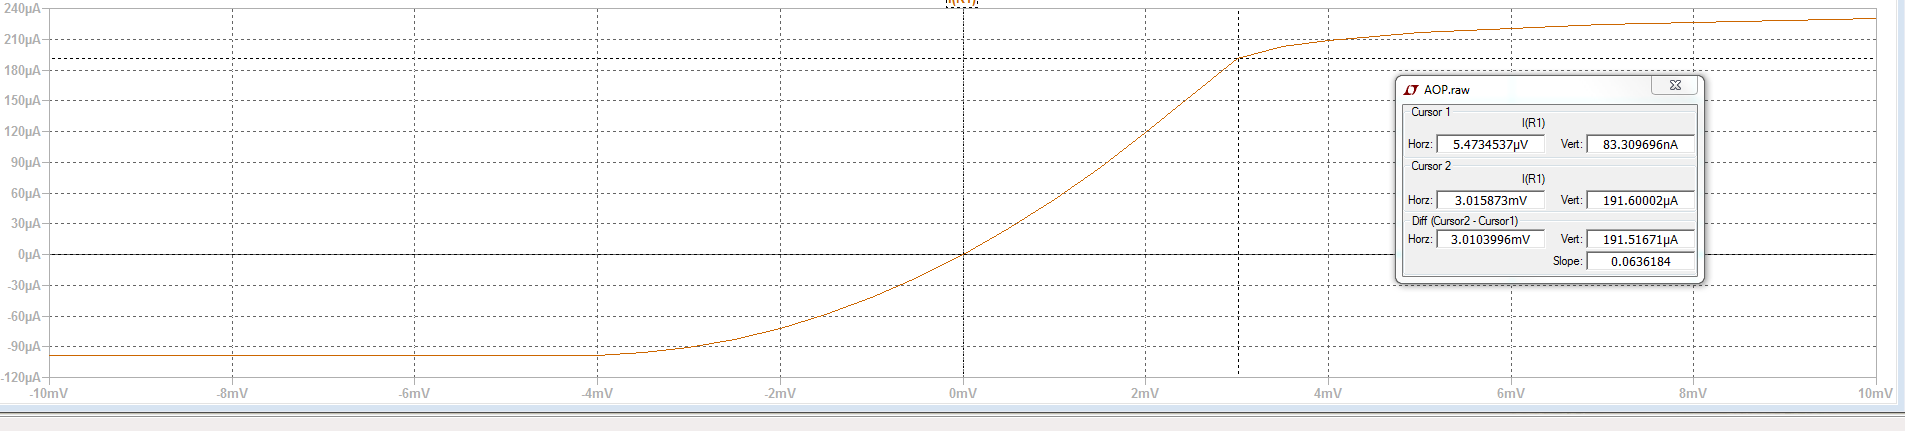
\includegraphics[width=\textwidth]{images/AopGm.PNG}
	\caption{Courant de sortie en fonction de la tension d'entrée}
	\label{fig:gm}
\end{figure}

La figure \ref{fig:gm} donne le courant de sortie en fonction de la tension d'entrée. On mesure une plage de fonctionnement linéaire comprise entre $-1 \; mV$ et $3 \; mV$. De plus, on mesure une transconductance de $64 \; mS$, ce qui est bien supérieur aux $10 \; mS$ initialement recherchés. On remarque également qu'il y a disymétrie dans la courbe obtenue. Ceci devra être corrigé en cas de poursuite de l'étude.

On mesure également le taux de réjection du mode commun $\tau = \frac{G_d}{G_c} = \frac{64 \; mS}{39 \; mS} = 1641$.

\newpage
\FloatBarrier
\newpage
\part*{Conclusion}

Ces deux séances de travaux de laboratoires nous ont permis de nous initier à la conception d'amplificateurs opérationnels. L'idée principale étant de réaliser un montage permettant de mesurer la différence de tension en entrée, ce qui est réalisé par l'étage 1, et d'amplifier fortement le signal obtenu grâce à l'étage 2.

Le montage obtenu est encore très largement perfectible, comme le montre la figure \ref{fig:gm}.


\end{document}